\chapter{Implementation}
The implementation phase of this project spanned across 9 weeks. Given that the software development methodology adopted was Extreme Programming. The platform was implemented with an iterative approach or a series of 'Weekly Cycles'. In this chapter, an overview of the work done in each weekly cycle will be provided, including a discussion of any problems encountered and how they were overcome.

As discussed in Section~\ref{process_ref}, at the beginning of each week it was decided which stories would be completed, with some non-essential stories included to add slack.

\begin{figure}[!htb]
	\centering
	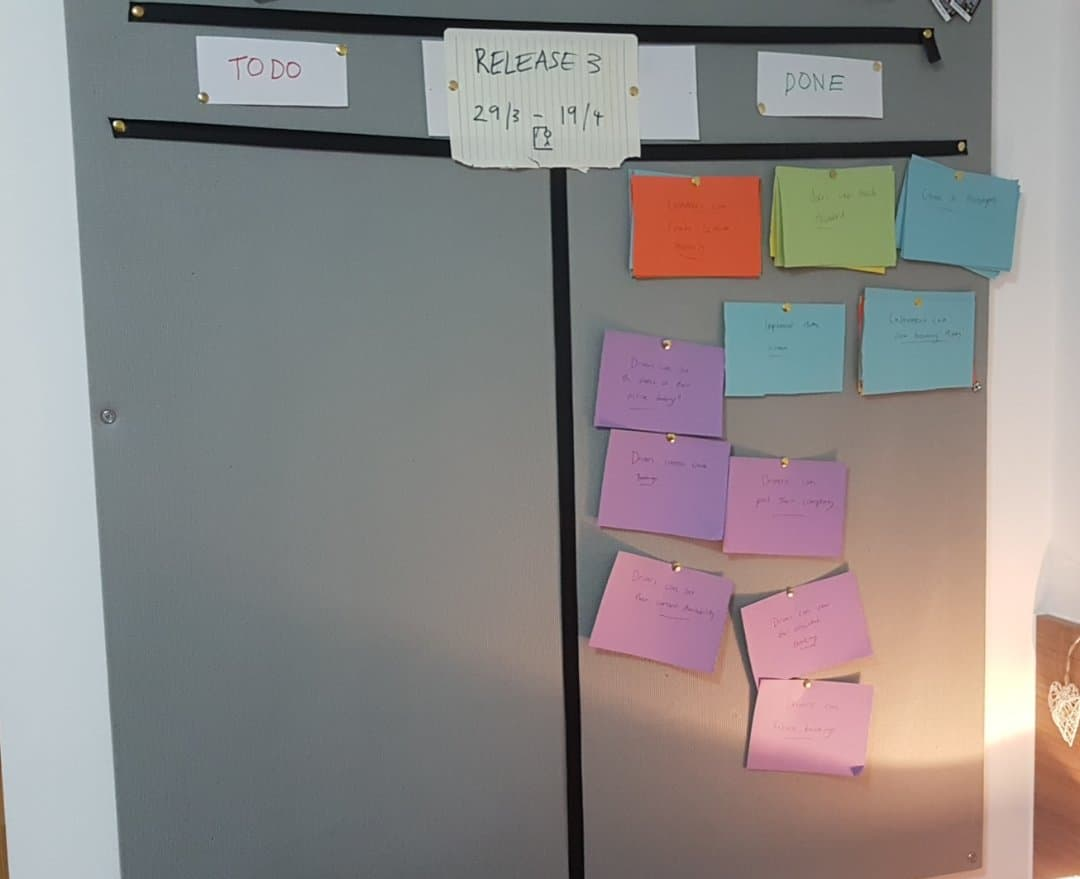
\includegraphics[width=0.5\linewidth]{Resources/img/story_board.jpg}
	\caption{The physical Story Board used throughout the project}
	\label{fig:story-board}
\end{figure}

\section{Week 1 (15/02 - 22/02)}
All the required prototyping for the platform took place in the first week of development. This included UI Prototypes for the Android App's screens, a prototype Authentication API, and a prototype Android App to consume the Authentication API.

\subsection{Prototype Authentication API}
During the creation of the prototype Authentication API, research into third-party authentication libraries was also done, with libraries such as Okta~\cite{okta_documentation_ref} and Passport.js~\cite{passport_documentation_ref} being considered. It was eventually decided, however, that a custom solution would allow for more fine-grain control over the API's authentication and access control.

\subsection{Prototype Android App}
Using the created API, the next task was to create a prototype Android App to consume the API. A major part of this task was to set up HTTP requests and JSON response de-serialization. The second tutorial in Raj Amal's series of walkthroughs~\cite{nodejs_authentication_tutorial_ref} proved essential in understanding Retrofit, rxJava, and Google's GSON. The prototype App allowed users to register, login, and view their profile. It enforced access control to ensure un-authenticated users couldn't view the main screen of the App. The Android aspect of this implementation was fairly trivial due to previous experience. For example, storing the user's access token in shared preferences and limiting access by requiring the presence of the token.

\subsection{User Interface Prototypes}
Now that there were prototypes in place to lay the foundation, it was time to prototype the User Interface for the actual platform. The first step in this process was to establish a general style and branding. This involved deciding on a colour scheme, choosing a typeface, and creating the first draft of the platform's logo. The remainder of the work involved actually creating the prototype for each of the App's screen. Prototypes were created with varying degrees of fidelity, the first pass simply involved sketching out some of the screens on paper. The final produced prototypes used Material Design components provided for Adobe XD~\cite{adobeXD_documentation_ref}. This meant that the produced prototypes would closely resemble the finished product produced in Android Studio. Examples of some of the created prototypes can be found in the report's appendices.

\begin{figure}[!htb]
	\centering
	\begin{subfigure}[b]{0.4\linewidth}
		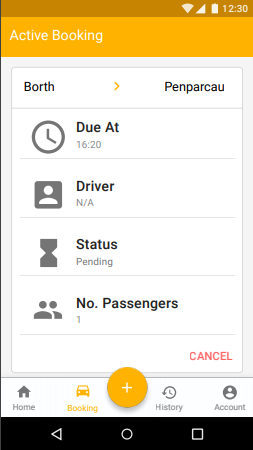
\includegraphics[width=\linewidth]{Resources/img/booking_overview_prototype.png}
		\caption{UI Prototype}
	\end{subfigure}
	\begin{subfigure}[b]{0.4\linewidth}
		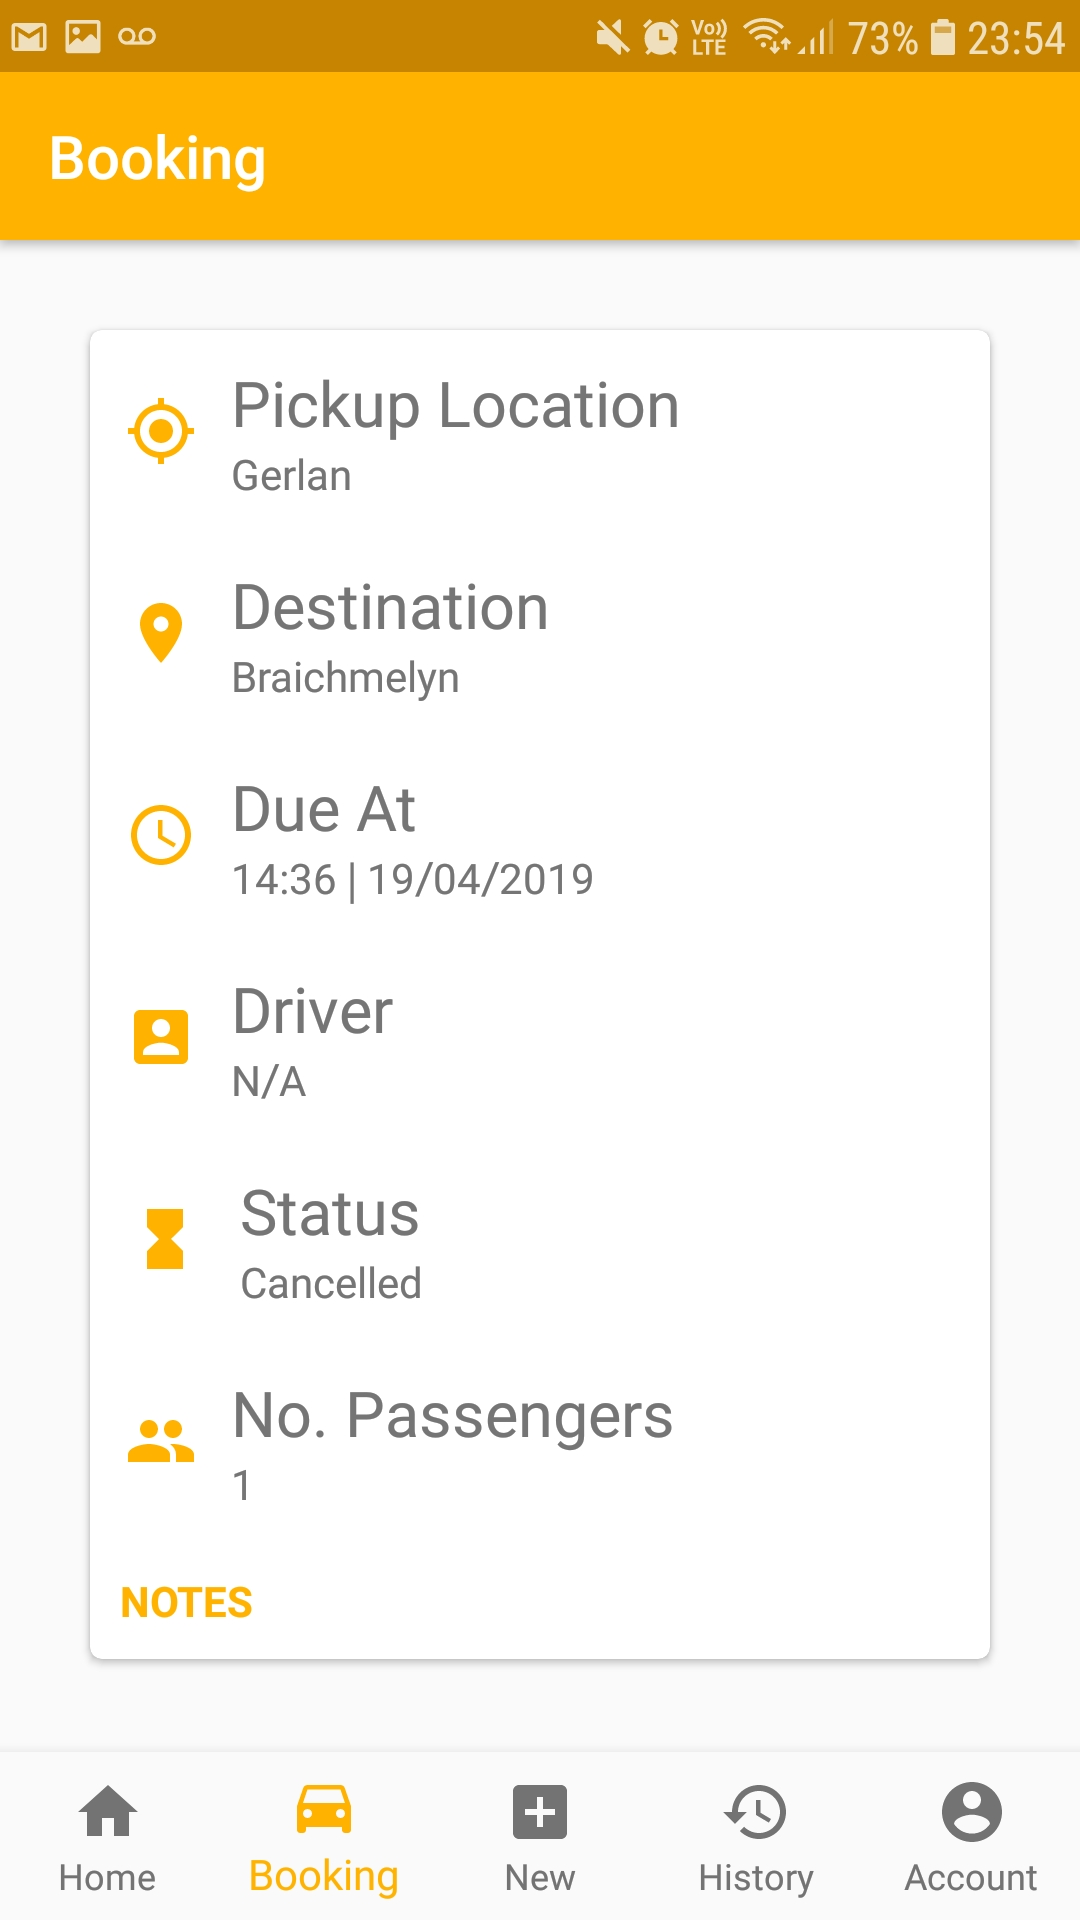
\includegraphics[width=\linewidth]{Resources/img/booking_overview_real.jpg}
		\caption{Actual Implementation}
	\end{subfigure}
	\caption{A comparison of the Booking Overview screen prototype and actual implementation}
	\label{fig:ui_compare}
\end{figure}

\newpage

\section{Week 2 (23/02 - 01/03)}
The focus of the second week of implementation was to get the REST API up and running and supporting all User related tasks: Registration, Authentication, and Account Management.

\subsection{Node.js Project Creation}
The very first step to implementing the API was to create the Node.js project and configure it to run in a Docker container alongside MongoDB. In order to create the Node.js project. An excellent GitHub repository~\cite{js_guidelines_documentation_ref} was discovered that outlined the best practices and standards in JavaScript projects.

\subsection{Containerization of Project}
Containerization of the API itself proved to be very straightforward, as it is a well-documented process and simply involved the creation of two files: Dockerfile and docker-compose.yml. The difficulty arose when attempting to connect the API container with MongoDB in order to persist data. The solution appeared to be to include a second container dedicated to MongoDB. This was working and a successful connection to the database could be made from within the API. However, in order to support data persistence after the containers were terminated, Data Volumes were required. A very helpful Medium tutorial~\cite{docker_medium_tutorial_ref} was used to correctly set up the data volumes and the setup was now working as intended.

\subsection{Authentication}
During the prototyping phase of development, an authentication API was created as a piece of spike work. Alongside this spike work, research into third-party authentication libraries was also done, with libraries such as Okta~\cite{okta_documentation_ref} and Passport.js~\cite{passport_documentation_ref} being considered. It was eventually decided, however, that a custom solution would allow for more fine-grain control over the API's authentication.

In order to provide the best security for the API, a token-based approach to authentication was used. It was also believed this would make the consumption of the API easier for the mobile application, by removing the need for sessions; thus making the API truly RESTful. The core principle behind this approach is that the user would send their email and password to a specific route within the API via Basic Authentication (Base64 encoding). The credentials would then be decoded and verified against the password hash stored in the database. If valid, the API would then provide the user with a 24-hour access token, to be sent in the header of any subsequent requests. Although initially requiring a bit of thought and research, implementation of this approach didn't provide any considerable difficulties. An excellent and in-depth tutorial written by Raj Amal~\cite{nodejs_authentication_tutorial_ref} was used as a reference to assist in the implementation.

\section{Week 3 (02/03 - 08/03)}
Testing of the API's current routes and consumption of the API by the Android App was the main focus of the third week.

\subsection{API Testing}
With the API already running inside a Docker container, the testing process was much more portable. Two testing libraries were used: Mochajs~\cite{mocha_documentation_ref} as the primary testing framework and Chaijs~\cite{chai_documentation_ref} as the assertation library. Whilst gaining familiarity with the testing libraries, Samuele Zaza's tutorial on Scotch.io~\cite{mocha_chai_tutorial_ref} was invaluable. The API was tested on a per-route basis, with several different cases for each route being tested. There was a bit of difficulty getting the tests to run seamlessly within the Docker container in TravisCI's environment. However, improved Docker Compose configuration eventually solve these issues, with assistance from Joe Cieslik's article in Hackernoon~\cite{docker_testing_tutorial_ref}.

\subsection{Implementation of Android App}
Consumption of the API by the Android App was where the bulk of the work took place during this week of development. Having already created a prototype App to consume an API using Retrofit and rxJava, much of the concepts and the boilerplate code was already in place. The difficulty came with refactoring the code to ensure reliability and good design practices. A major part of this was the implementation of the Model, View, ViewModel design pattern. An article on Medium.com by Ahmad Shubita~\cite{mvvm_tutorial_ref} was used to get to grips with the design pattern and its implementation via Retrofit.

Another essential aspect of the consumption of the API by the Android App was Error Handling, this is especially true for the registration process. In order to fully support internationalization/localization within the app, it was important that English error messages from the API not be displayed directly to the UI. Rather that error responses from the API come with four attributes: 'name' - the name given to a particular error; 'code' - an arbitrary number associated with a given error; 'message' - the error's name displayed in a more human-readable way; and 'description' - a brief description of the nature of the error. This way, the mobile app that consumes the API can simply read the code associated with a given error and fetch the matching string resource. One notable downside to this approach is that it increases the maintenance required. For example, if updates are made to the API that affects its error handling (a new error is added), this change must be accounted for in the App's Error-Parser.

\begin{figure}[!htb]
	\centering
	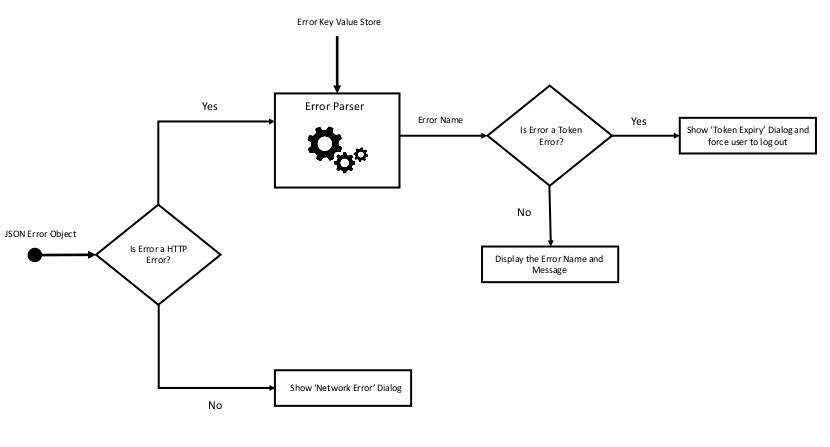
\includegraphics[width=\linewidth]{Resources/img/error_handling_flowchart.png}
	\caption{A flowchart depicting the error handling process within the Android App}
	\label{fig:error_flowchart}
\end{figure}

\section{Week 4 (09/03 - 15/03)}
The fourth week of development was mainly focused on preparations for the mid-project demonstration. Therefore, implementation of the platform itself was halted.

\subsection{App Deployment}
A major part of the preparations required for demonstrating the app's progress so far was the deployment of the API. Up to this point, the App had only been usable within an emulator ran on the same machine as the Node.js application. In order to properly demonstrate the app's development, it had to be able to access the API from an actual mobile device.

As discussed in Section~\ref{deployment}, it was decided that the API would be deployed on a local server box using the Node.js process manager and Nginx's reverse proxy. Although there are certainly benefits to using Docker in production, for example, reduced setup times and improved portability. Much of the research done heavily discouraged its use if inexperienced, especially in a self-hosted environment. Therefore, the decision was made to deploy the API without docker, however, it will continue to be utilized for development and testing environments.

The majority of the steps required to deploy the API were fairly straightforward and very well documented~\cite{deployment_tutorial_ref}. As discussed previously, there are certainly security implications associated with the chosen deployment approach. Such as lack of decent support for SSL, physical security concerns, inexperience with system administration, and the server itself being used for other, unrelated web applications. However, as a solution for demonstration purposes with fictitious personal data, it served its purpose excellently.

\section{Week 5 (16/03 - 22/03)}
With authentication already completed and supported both in the mobile app and on the REST API, the next logical step was to work on the implementation of booking creation. This task took surprisingly less time than anticipated, therefore there was time to complete some of the 'slack tasks'.

\subsection{Booking Data Model support whithin the API}
Having already implemented user authentication, creation, and management within the API, much of the foundations required for booking creation, management, and viewing were already in place. The main steps required were the following:

\begin{itemize}
	\item Create booking model
	\item Interact with booking model via service
	\item Create a controller to allow the router to interact with the service
	\item Implement all the necessary routes for bookings (CRUD)
	\item Add all the required input validations and error handling
	\item Write unit tests for each booking route
\end{itemize}

The booking model, service, controller, and router are all fairly standard and similar to those for the user data model. 

Input validation for booking creation was fairly trivial, with the exception of the 'time' field, as it had some special constraints:

\begin{itemize}
	\item Booking time cannot be further than 3 hours in the future
	\item Boking time cannot be sooner than 10 minutes away
	\item Booking time cannot be in the past
\end{itemize}

In order to easily compare time values, the ISO 8601 time stamp had to be parsed into a plain Javascript date object.

\subsection{Booking Creation support within the Android App}
Similarly to the API, having full support for the user data model within the App already made the implementation of booking creation very straightforward. Aspects of the App such as error handling and validation had to be updated to support the changes in the API.

The main challenge for this aspect of the implementation was the UI. A dedicated Activity was created for booking creation, with standard text inputs for pickup location, destination, and notes. The number of passengers and booking time fields each have a custom dialog that prompts the user for an input. The number of passengers dialog is a custom dialog that contains a number-picker, with the parent activity implementing its value listener. Therefore, whenever the value of the number picker is changed, the parent activity is kept updated. The time picker, however, is a default android time picker with the dialog all created programmatically. Therefore, tracking the selected value was trivial.

An interesting challenge faced when implementing the booking creation activity was deciding how to force the App to navigate to the 'booking viewing' screen upon successful creation of a booking. A considered option was simply to force the navigation whenever the booking creation activity was closed. However, this would prompt navigation even when the booking creation was canceled, which was an undesired behavior. The solution eventually implemented was to launch the booking creation activity with Android's 'startActivityForResult()' method. This would allow the activity to provide a return code when exited, meaning the activity could either exit with success or failure. If exited with success, a toast message is shown and the navigation is changed.

\subsection{Account Management within the Android App}
As mentioned at the start of this section, the primary tasks for this week's implementation took less time than anticipated. Therefore there was time to implement some of the less essential features. 

Given that the support for account management was already supported in the API, it made sense to create the UI for account management. The main features of the account screen are a circular avatar with the user's first name initial and a list of account actions. All of the account actions were implemented with the exception of changing password. This required further security precautions within the API.

\subsection{Support Dynamic Orientation within the Android App}
The next functionality to be addressed was landscape support, up until this point the app had been locked into portrait mode for simplicity. Most screens ported over to landscape fairly easily, given that the Constraint Layout was used for most screens and is typically well supported in both landscape and portrait modes. However, the account overview screen required its own layout file specifically for landscape mode. Luckily, Android makes this very easy with the use of the 'land' suffix in resource folder names. A new resource folder named 'layout-land' was created to contain the landscape specific layout. 

Allowing the app to be rotated did present some unexpected complications,  specifically concerning asynchronous API calls. When a fragment or activity is destroyed, any outstanding asynchronous subscriptions are terminated (to avoid dangling). This does, however, mean that whenever a view is destroyed and re-created due to orientation change, any outstanding API calls are discarded. A simple, yet arguably lazy solution to this issue was simply to lock the orientation in place whenever an API call is made, then to unlock the orientation upon completion.

\subsection{Welsh Language Support within the Android App}
Having gone to the effort to support internationalization/localization within the app, it made sense to add string values for another language. This was trivial and simply involved translating all the existing string values and adding them to a '-cy' resource directory.

\section{Week 6 (23/03 - 29/03)}
This week's development was almost entirely based on the Android App. It primarily involved full support for bookings via implementation of the following: Active Booking Overview, Booking Cancelation, Booking History. Password changing was also re-visited.

\subsection{Active Booking Overview}
The user's currently active booking could be retrieved by simply retrieving their most recent booking. This is guaranteed to be accurate as new bookings cannot be created whilst an active booking already exists. The booking overview screen simply contained a card view with information populated by the API request. The card view is populated using Android's Data Binding library, allowing for stricter conformity to the MVVM design pattern.  Unfortunately, the view does need to be manually refreshed to fetch up to date data. However, this is made intuitive through the use of Android's SwipeRefreshLayout. The view is also refreshed whenever the user changes navigation.

\subsection{Booking Cancelation}
After implementing the booking overview screen, adding support for booking cancelation was trivial. A text-button was added to the bottom of the card view. Pressing the button prompts a simple confirmation dialog to the user. If confirmed, a request is sent to the API to update the booking's status to 'Cancelled'.

\subsection{Booking History and Custom JSON De-Serialization}
As seen in Figure~\ref{fig:entity_relationship}, the way bookings are stored under a user's record in the database is as an array of MongoDB Object IDs. Therefore when a user is retrieved from the API, their bookings are shown simply as a list of Object references. Whereas the booking history list is required to display a limited amount of information about the booking. Although technically each booking could be retrieved fully by making a GET request to the API for that specific booking, this is an undesirable solution and would require significantly more API requests. Therefore a new route was implemented within the API specifically to retrieve a full list of a user's bookings. Mongoose's 'populate' function proved very useful for this purpose. 

The newly created route does not populate the 'driver' and 'customer' fields of the booking. Meaning they are still represented as strings (object IDs), whereas the booking model within the App stores the driver and customer fields as User objects. This caused some unexpected complications when it came to de-serialization of the JSON booking objects. When the booking JSON object was returned from a GET request to the /bookings/ route, it would be de-serialized just fine (due to driver and customer being populated). Whilst, if the booking JSON objects were returned from the /users/{id}/bookings route, a de-serialization exception was thrown. Upon further research, it was discovered that custom GSON de-serializers could be created that accounted for dynamic JSON fields. Although it took some time, this was done relatively easily and the problem was resolved.

The remainder of the implementation for booking history went off without a hitch, a boilerplate Recycler View Adapter was created to handle the list of bookings. With a click listener to open an Activity and display the booking's full details. The booking overview fragment created earlier in this section was re-used here.

\subsection{Password Changing}
All of the UI elements required for supporting password changing were already implemented. An update to the user updating route on the API was required in order to force the user to provide a valid previous password before the changes could be approved.

\section{Week 7 (30/03 - 05/04)}
This week's primary focus was adding support for the Driver role within the platform. There was also some time to implement the app's home screen and re-assess how notes were being handled within bookings.

\subsection{Supporting the Driver Role}
In order to fully support drivers within the API, a few changes needed to be made. The User model had to be updated to include fields for the driver's availability and company. This was fairly straightforward and simply required the addition of the fields to the model file and support for their update in the PATCH route. Some extra authorization checks were required for the user PATCH route, to ensure a user would only be able to change their own role under specific circumstances (resignation from a company).

All other aspects of the user model were already designed to accommodate users of different roles. For example, the 'bookings' field required no change as it could serve different purposes depending on the user's role. 

It was also predicted that certain routes in the future would need to be 'role-protected'. Therefore a very simple role-based access control middleware was created. The middleware could be applied to any route and either a single role or a list of roles could be authorized for that given route.

\subsection{Redesign of the Booking Notes System}
Having initially opted that a booking's notes be a single, optional string. It was decided that the support for communication this provided was very minimal. It's only purposed so far was to allow a Customer to make 'special requests' along with their booking. However, it was realized that a collection of notes within a booking that could be added by both the Customer and the Driver could potentially serve as a very simple communication mechanism. Notes would also be added by the system itself to inform users when changes to their booking have occurred, for example, status changes.

Implementing the new booking notes system on the API was very straightforward, it simply required a different type within the Booking model; together with support for appending notes to a Booking via its PATCH route.

\subsection{The App's Home Screen}
The last bit of development for this week of implementation was the fairly small task of implementing a home screen for the app. The layout and contents of this screen were decided a long time ago in the prototyping phase. Therefore the only required work was creating the screen's XML layout for both portrait and landscape orientations and implementing the API requests required. The information needed for the home screen required two requests be made to the API: one for the user's information (name, role, number of bookings) and another for the user's most recent booking information.

\section{Week 8 (06/04 - 12/04)}
This was the last week of development on the Android App, quite a lot of functionality was added. Primarily, complete support for Drivers within the App and updates to the booking overview to support the new notes system. In addition to developments within the App itself, it was also required that preparation work be done in the API, to support the Company Admin Web App.

\subsection{Supporting the new Notes System within the App}
In order to support the new notes system that was developed in the previous week,  a new Activity was created to serve as a 'notes view'. This new activity also contained a Floating Action Button that opened a text input for the user to append a new note to the booking. The only minor obstacle encountered in this implementation was that notes were simply an array of strings with no date stamp. Therefore in order to display them in semi-chronological order, the returned array was reversed (as they were being appended to the back of the array within the database).

\subsection{Implementing all the Driver Featuress within the App}
In order to implement all the functionality required for drivers within the app, surprisingly little work had to be done. The main tasks involved: The addition of an availability switch; an option to resign from their company; removal of 'booking creation'; support for viewing several active bookings; and support for updating a booking's status.

The addition of an availability switch and resignation option was fairly straightforward, the most difficult aspect was displaying an alternative 'home screen' and 'account overview' depending on the user's role. This was done by storing the user's role in the App's shared preferences and using this value to determine what version of each dynamic screen was loaded.

The API had already been updated to prevent drivers from creating bookings, however, the navigation option and booking creation screen were still very much available. It was decided that simply removing the 'new booking' option within the app's navigation for Drivers was the best solution. This was achieved with the addition of a second XML navigation menu, the required menu was then loaded into the Navigation Bar as needed. If the user opted to resign as a driver from within the App itself, the dynamic aspects of the app such as the Navigation Bar, Home Screen, and Account Screen were automatically changed to 'Customer Mode'. However, if the user was forcibly 'demoted' by their Company's Management, the App would not automatically update the required screen. 

Although still not ideal, the best conceivable solution was to query the user's role whenever a request is made to the API. This is when the most up-to-date information regarding the user is retrieved and the App could then select the correct 'mode' to display. However, unavoidably, the user's token would still contain a payload that indicated their role was 'Driver'. Therefore any attempt at the booking creation would be rejected. This problem would also persist if the order of role change was the other way around (Customer to Driver). It was ultimately decided that if the App detected any change in the user's role, it would consider the user's 'session' as expired and log them out.

The final step required in order to fully support Drivers within the app was implementing the ability to view multiple active bookings at once and edit their status. Whilst implementing the Customer aspects of the app it was assumed that only one active booking could exist at any given time. However, there was already support for 'booking lists' (due to the History screen). Therefore the approach was to re-use the Recycler View Adapter used by the Booking History list and implement a new view for each 'entry'. Upon clicking on an entry in the active booking list, the original Booking Overview fragment could also be re-used to display details about the booking. However, some amendments had to be made to the Booking Overview fragment for it to be usable by Drivers, namely: Replacing the 'Driver' field with 'Customer', and the addition of an 'edit' button by the booking's status. Of course, these changes would only be available to Drivers. The Booking Overview fragment would use the same approach as the other 'dynamic' screens within the app in order to display the correct content based on the user's role.

\subsection{Implementing the Company Model within the API}
In preparation for the development of the Web Application that is targeted towards Company Admins, the API had to be adapted to support Companies. Because most of the design for Company support had already been conceptualized, implementing the model for the Company was fairly straightforward. The same steps required for implementing Users and Bookings were taken, including the creation of a model, controller, and service file. With all the required /companies/ routes also implemented.

The bulk of the work took place in deciding how Companies would receive bookings from Customers. In the early stages of development, it was hoped that bookings would be delegated to companies automatically, by the system. However, for simplicity and to give full control to the companies themselves, a virtual 'booking market' approach was selected. This would include a list of all unallocated bookings that have been created by Customers. A Company Admin can then view this list and chose to 'claim' a booking. Once claimed, the booking would be removed from the list and would have all the object references required to 'belong' to that company. The same principle would apply for allowing companies to 'release' a booking, back into the 'booking market'. This would effectively undo all of the object references from the 'claiming' process.

The above mechanisms were implemented through the addition of three new routes: GET /bookings/, PATCH /bookings/{id}/release, PATCH /bookings/{id}/claim. The routes have all the necessary access protections to ensure only authorized users can perform the actions (for example, bookings can only be released by the company that owns it).

\section{Week 9 (13/04 - 19/04)}
The final week of development focused solely on the implementation of the Responsive Web App. In order to serve some of the created screens within the Web App, some minor updates to the API were also required.

\subsection{Web App Implementation}
Although the primary focus during the prototyping phase was on the API and the Android App itself. Some low-fidelity pen and paper UI prototypes were also created for the Web App. It was eventually decided, however, that the best choice for the Web App's User Interface was to use a template~\cite{angular_material_documentation_ref}. This shaved off a lot of implementation time (that was becoming scarce at this point of development) and also provided a professional, consistent look and feel. Having used a Material Design template, it also matched the style that was established throughout the development of the Mobile App.

Thankfully, most use-cases for the Web App required only boilerplate Angular code to make requests to the API and display the results on the screen. Bootstrap tables were mostly used to display information. Authentication and Access Control mirrored what had been done on the mobile app, with the user's access token being stored in local storage and attached to any HTTP request headers. Error Handling was also very straightforward, with any errors simply being displayed to the user via a notification element. The only downside to this approach is that error messages were being shown directly from the HTTP response, making the Web App unfriendly for internationalization. This is an area that given an opportunity for further development, would certainly be addressed.

\begin{figure}[!htb]
	\centering
	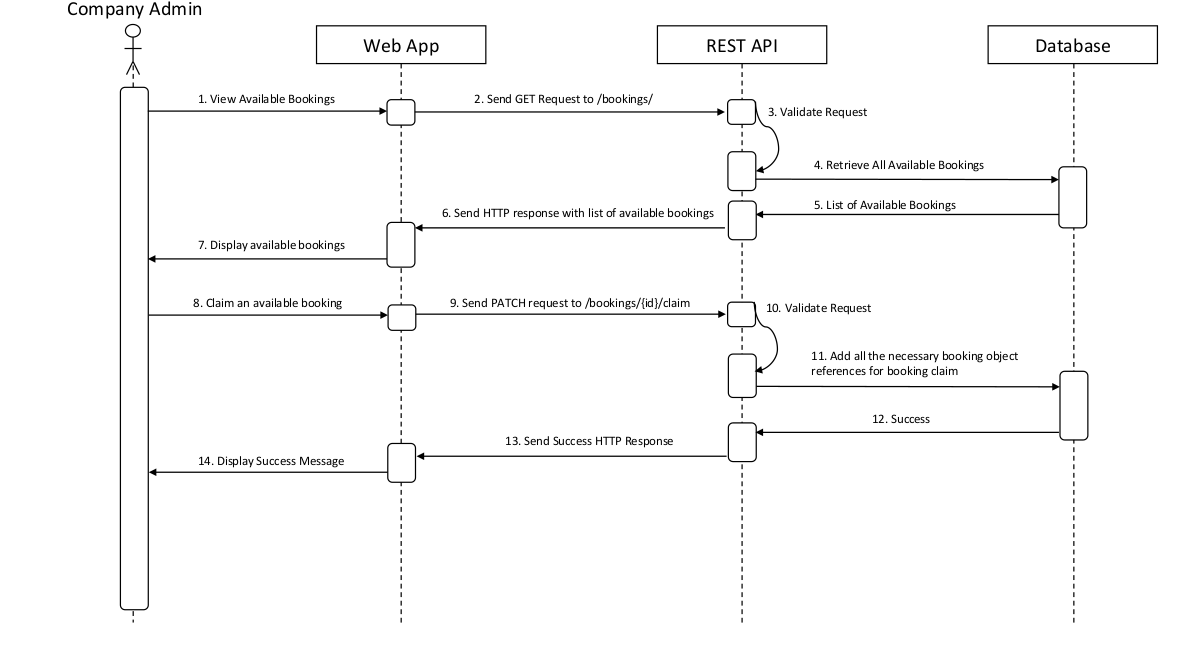
\includegraphics[width=\linewidth]{Resources/img/booking_claim_sequence.png}
	\caption{A UML Sequence Diagram showing the process of claiming a booking via the Web App}
	\label{fig:booking_claim_sequence}
\end{figure}

\subsection{Required Updates to the API}
Some aspects of the Web App's development called for changes to the API in order to be implemented successfully. The two most prominent examples are listing of a Company's Admins and recruiting drivers via their email. There was no dedicated mechanism within the API to retrieve a populated list of a Company's Admins, this was required for the Web App's 'company profile' screen. This addition was very simple and simply involved the creation of a new route 'GET /companies/{id}/admins' that retrieved a list of admins.

Another required change was supporting the addition of drivers to a company by their Email. Up to this point, Drivers had been added to a company by their Object IDs. However, this was not ideal, as Object IDs are long, complex strings that a user is unlikely to memorize or have access to. Therefore the 'PATCH /companies/drivers' route was adapted to support user emails as opposed to Object IDS.

